\documentclass[11pt]{article}
\usepackage[a4paper,landscape,margin=1.2cm]{geometry}
\usepackage{graphicx}
\usepackage{tikz}
\usetikzlibrary{calc}

\pagestyle{empty}

\begin{document}

\begin{center}
\resizebox{\textwidth}{!}{%
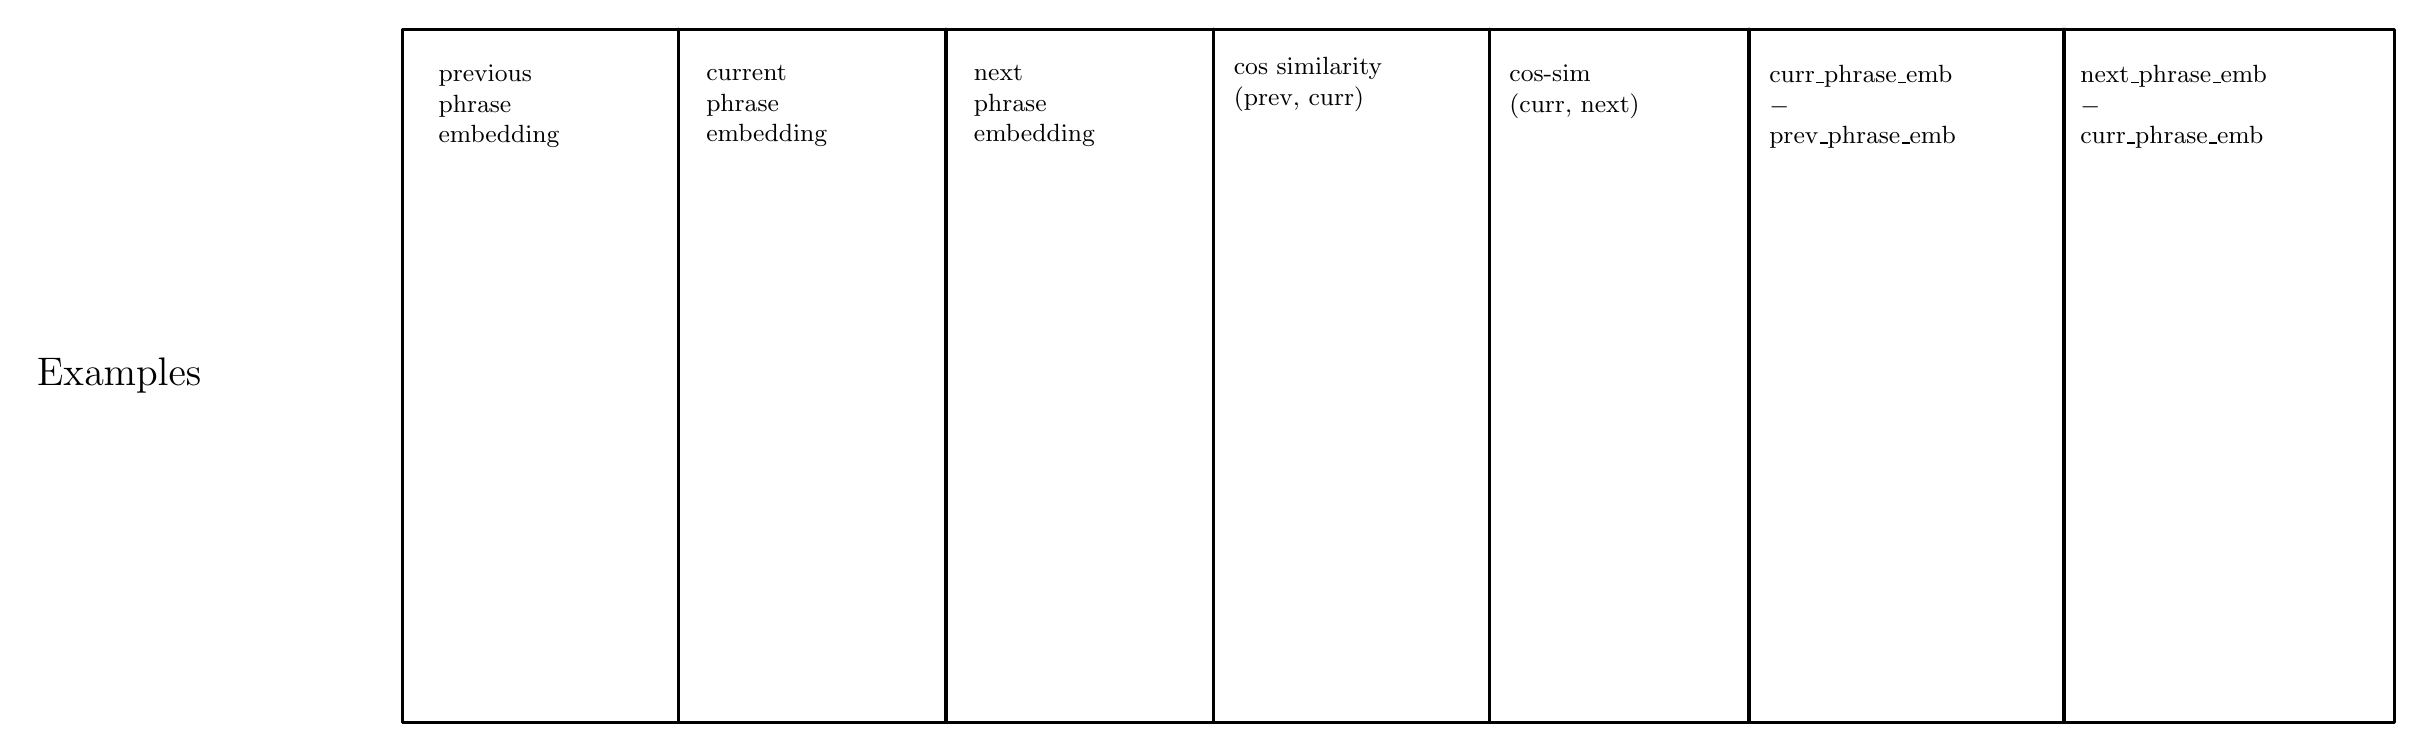
\begin{tikzpicture}[
    x=1cm,
    y=1cm,
    line cap=round,
    line join=round,
    header/.style={
        anchor=north west,
        align=left,
        font=\small,
        inner sep=0pt,
        text depth=0pt
    }
]
    % Table geometry
    \def\tableheight{8.8}
    \def\leftlabeloffset{3.6}

    \pgfmathsetmacro{\xA}{0.0}
    \pgfmathsetmacro{\xB}{3.5}
    \pgfmathsetmacro{\xC}{6.9}
    \pgfmathsetmacro{\xD}{10.3}
    \pgfmathsetmacro{\xE}{13.8}
    \pgfmathsetmacro{\xF}{17.1}
    \pgfmathsetmacro{\xG}{21.1}
    \pgfmathsetmacro{\xH}{25.3}

    % Outer border
    \draw[very thick] (\xA,0) rectangle (\xH,\tableheight);

    % Column separators
    \foreach \x in {\xB,\xC,\xD,\xE,\xF,\xG} {
        \draw[very thick] (\x,0) -- (\x,\tableheight);
    }

    % Left-side row label, placed outside the table as in the sketch.
    \node[font=\Large] at ($(\xA,0.5*\tableheight)+(-\leftlabeloffset,0)$) {Examples};

    % Header text
    \node[header, text width=2.8cm] at (\xA+0.45,\tableheight-0.45)
        {previous\\phrase\\embedding};

    \node[header, text width=2.8cm] at (\xB+0.35,\tableheight-0.45)
        {current\\phrase\\embedding};

    \node[header, text width=2.8cm] at (\xC+0.35,\tableheight-0.45)
        {next\\phrase\\embedding};

    \node[header, text width=2.8cm] at (\xD+0.25,\tableheight-0.35)
        {cos similarity\\(prev,\ curr)};

    \node[header, text width=2.6cm] at (\xE+0.25,\tableheight-0.45)
        {cos-sim\\(curr,\ next)};

    \node[header, text width=3.3cm] at (\xF+0.25,\tableheight-0.45)
        {curr\_phrase\_emb\\$-$\\prev\_phrase\_emb};

    \node[header, text width=3.4cm] at (\xG+0.20,\tableheight-0.45)
        {next\_phrase\_emb\\$-$\\curr\_phrase\_emb};
\end{tikzpicture}%
}
\end{center}

\end{document}
